\begin{figure}[ht!]
    \centering
    % \begin{tabular}[c]{ccc}
    % \begin{subfigure}[c]{0.31\textwidth}
    %     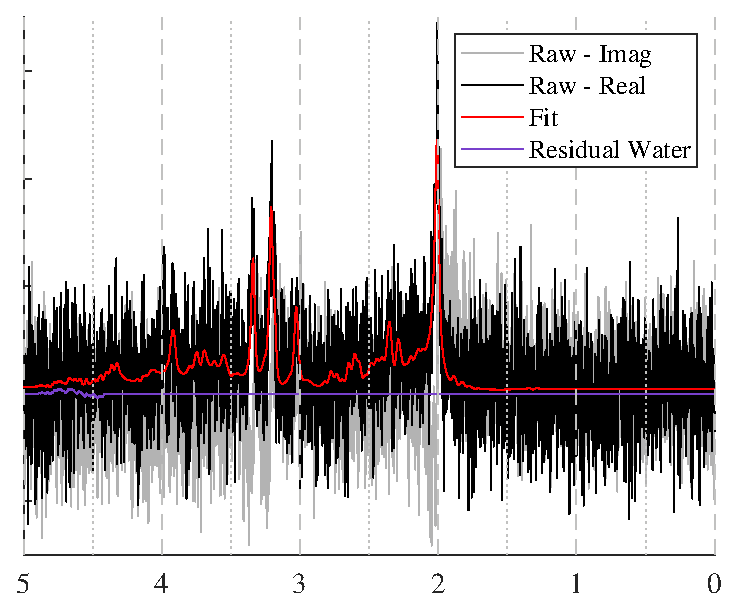
\includegraphics[width=0.93\textwidth]{images/samples_by_artifact/30ms_artifact_samples_snr_1.eps}
    %     \caption{Spectral SNR=2}
    %     \vspace{3pt}
    % \end{subfigure}&
    % \begin{subfigure}[c]{0.31\textwidth}
    %     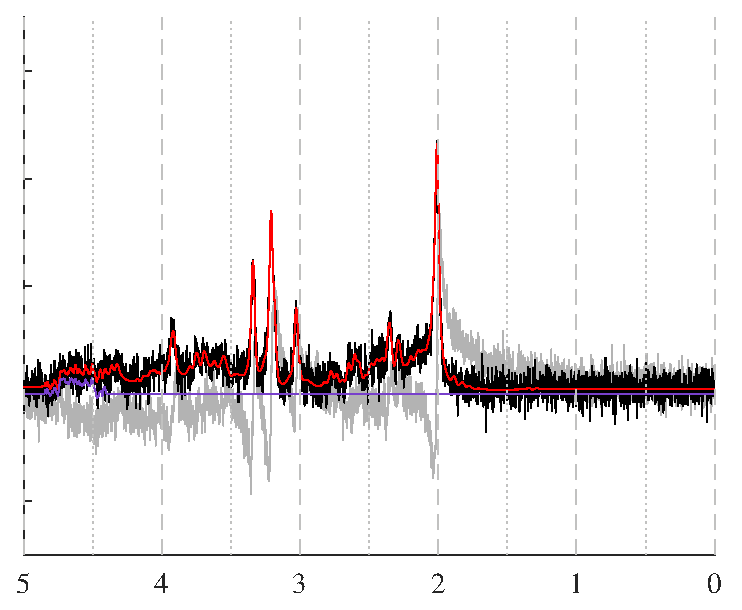
\includegraphics[width=0.93\textwidth]{images/samples_by_artifact/30ms_artifact_samples_snr_2.eps}
    %     \caption{Spectral SNR=8}
    %     \vspace{3pt}
    % \end{subfigure}&
    % \begin{subfigure}[c]{0.31\textwidth}
    %     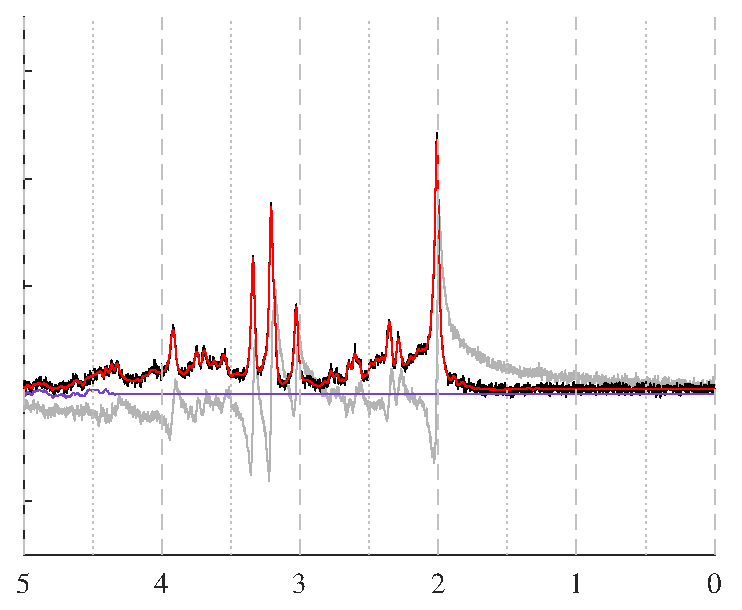
\includegraphics[width=0.93\textwidth]{images/samples_by_artifact/30ms_artifact_samples_snr_3.eps}
    %     \caption{Spectral SNR=14}
    %     \vspace{3pt}
    % \end{subfigure}\\
    % \begin{subfigure}[c]{0.31\textwidth}
    %     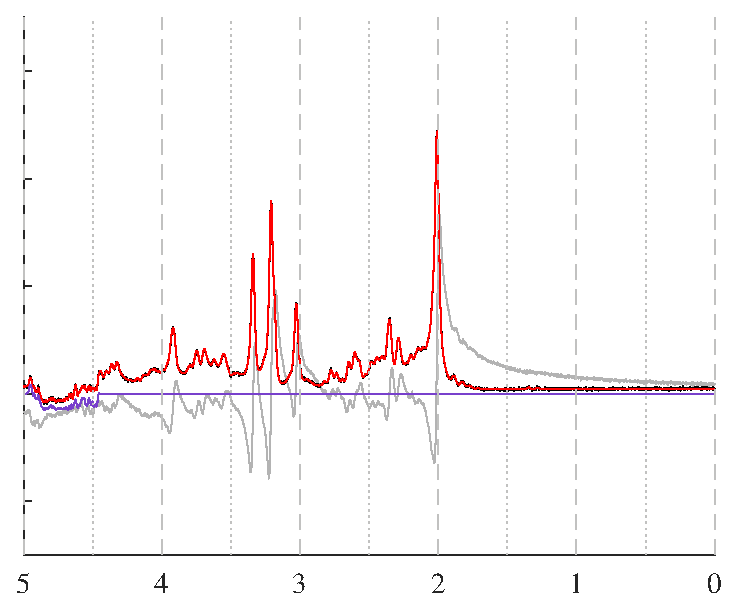
\includegraphics[width=0.93\textwidth]{images/samples_by_artifact/30ms_artifact_samples_snr_4.eps}
    %     \caption{Spectral SNR=20}
    %     \vspace{3pt}
    % \end{subfigure}&
    % \begin{subfigure}[c]{0.31\textwidth}
    %     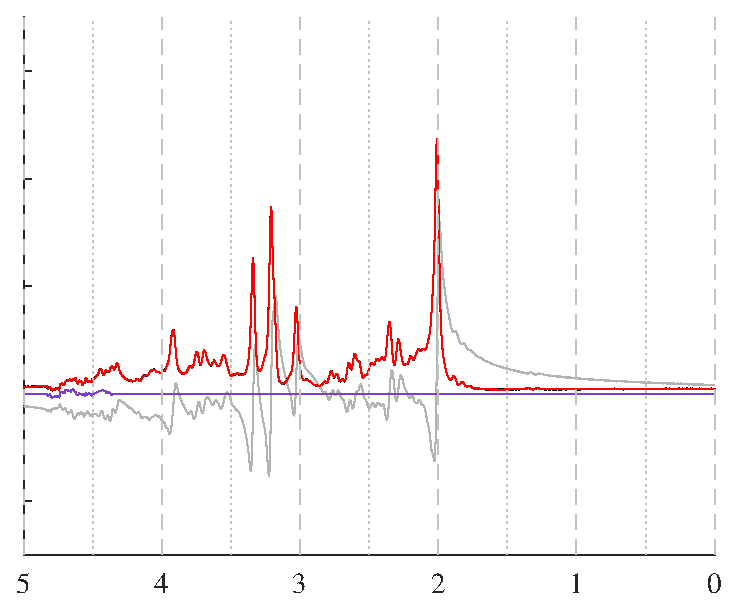
\includegraphics[width=0.93\textwidth]{images/samples_by_artifact/30ms_artifact_samples_snr_5.eps}
    %     \caption{Spectral SNR=26}
    %     \vspace{3pt}
    % \end{subfigure}&%
    % \begin{subfigure}[c]{0.31\textwidth}
    %     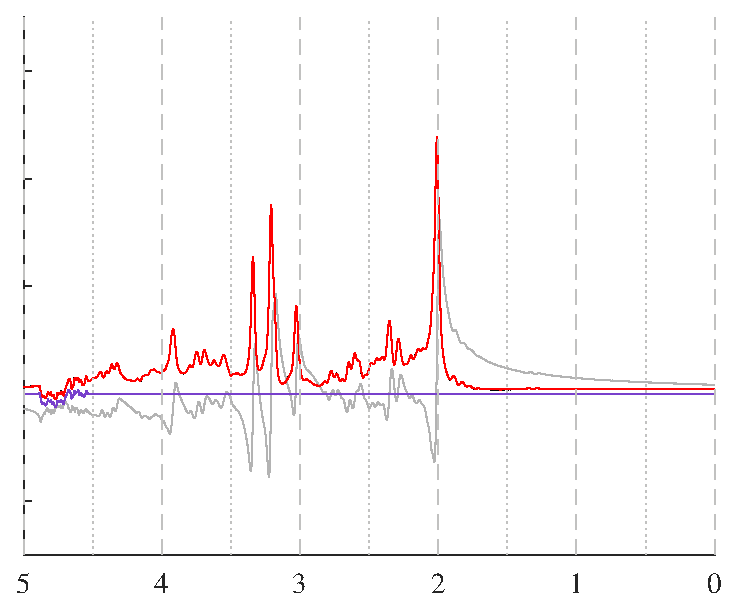
\includegraphics[width=0.93\textwidth]{images/samples_by_artifact/30ms_artifact_samples_snr_6.eps}
    %     \caption{Spectral SNR=32}
    %     \vspace{3pt}
    % \end{subfigure}\\
    % \end{tabular}
    \includegraphics[width=\textwidth,keepaspectratio]{images/compiled_figures/MRS_Sim_Figure_14_SNR_samples.png}
    \caption{Identical spectra are displayed with varying spectral SNRs as indicated below each plot. The lorentzian broadening was left unscaled and the gaussian broadening = 20 Hz. All phase offsets and eddy currents were omitted.}
    \label{fig:30ms samples snr}
\end{figure}

